% Poly Citra CoolBrick: KVRSS SPARK Innovation Awards application
% Compile with: pdflatex poly_citra_coolbrick_kvrss.tex  (run twice)
\documentclass[11pt,a4paper]{article}
\usepackage[a4paper,margin=2cm,bottom=2.2cm]{geometry}
\usepackage[T1]{fontenc}
\usepackage[utf8]{inputenc}
\usepackage[scaled=0.95]{helvet}
\renewcommand{\familydefault}{\sfdefault}
\usepackage{textcomp}
\DeclareUnicodeCharacter{20B9}{Rs\,}
\usepackage{xcolor}
\usepackage{graphicx}
\usepackage{booktabs}
\usepackage{tabularx}
\usepackage{array}
\usepackage{enumitem}
\usepackage{titlesec}
\usepackage{fancyhdr}
\usepackage[most]{tcolorbox}
\usepackage{float}
\usepackage{needspace}
\usepackage{caption}
\captionsetup{font=small,labelfont=bf}
\usepackage{pgfplots}
\pgfplotsset{compat=1.18}
\usepackage{hyperref}
\graphicspath{{img/entry/}}

\definecolor{accent}{HTML}{C0571A}
\definecolor{ink}{HTML}{2B2B2B}
\definecolor{blue}{HTML}{2F6E9E}
\definecolor{pale}{HTML}{FBF1EA}
\color{ink}
\hypersetup{colorlinks,urlcolor=blue,linkcolor=ink}

\setlength{\parindent}{0pt}
\setlength{\parskip}{6pt}
\linespread{1.08}

% ---- the 8 required sections: highlighted bars --------------------------
\newcommand{\sectionbar}[1]{\begin{tcolorbox}[enhanced,colback=accent,colframe=accent,arc=3pt,boxrule=0pt,
     left=8pt,right=8pt,top=5pt,bottom=5pt,before skip=0pt,after skip=0pt,fontupper=\Large\bfseries\color{white}]
   \thesection.\enspace #1\end{tcolorbox}}
\titleformat{\section}[block]{\needspace{5\baselineskip}}{}{0pt}{\sectionbar}
\titlespacing*{\section}{0pt}{10pt}{-6pt}
\titleformat{\subsection}{\large\bfseries\color{accent}}{}{0pt}{}
\titlespacing*{\subsection}{0pt}{8pt}{0pt}

\newtcolorbox{usp}{enhanced,colback=pale,colframe=accent,boxrule=1.2pt,arc=4pt,
  left=10pt,right=10pt,top=10pt,bottom=8pt,title={\bfseries OUR USP},fonttitle=\small,
  coltitle=white,colbacktitle=accent,attach boxed title to top left={yshift=-2.2mm,xshift=10pt},
  boxed title style={arc=2pt,boxrule=0pt}}

\newcommand{\pic}[2]{\begin{minipage}[t]{0.32\textwidth}\centering
  \includegraphics[width=\linewidth,height=3.1cm,keepaspectratio=false]{#1}\\[2pt]
  {\small\bfseries #2}\end{minipage}}

\pagestyle{fancy}\fancyhf{}\renewcommand{\headrulewidth}{0pt}
\fancyfoot[R]{\small\color{gray}Poly Citra CoolBrick \textbullet\ \thepage}

\begin{document}

% ---- application details --------------------------------------------------
{\fontsize{30}{34}\selectfont\color{blue!60!black} Poly Citra CoolBrick}\par
\vspace{2pt}{\color{blue}\rule{\textwidth}{0.8pt}}\par
\vspace{4pt}
\renewcommand{\arraystretch}{1.5}
\begin{tabularx}{\textwidth}{@{}>{\bfseries}p{4.6cm}X@{}}
\toprule
Field & Rasayanam (Chemistry) \\
Title of the Project & Poly Citra CoolBrick \\
Name of the Student(s) & Daiwik Abrol and Rian Sikka \\
Class & Grade 9 (IGCSE) \\
School & Scottish High International School \\
Simulation Video & \url{https://youtu.be/kSh3PBh7VoA} \\
\bottomrule
\end{tabularx}
\renewcommand{\arraystretch}{1}
\vspace{6pt}

% =========================================================================
\section{Summary (A brief overview of project in English)}
A box of broken Styrofoam takes up a surprising amount of space. Most of that
volume is air. We used D-limonene extracted from discarded orange peels to
dissolve the foam. As the air escaped, the foam collapsed into a thick gel
that we could press into a mould and cure into a solid brick sample.

\medskip
\noindent\pic{foam.jpg}{Discarded foam packaging}\hfill
\pic{peels.jpg}{Discarded orange peels}\hfill
\pic{sample.jpg}{Our cured brick sample}

We are studying whether this waste-derived material could also slow the heat
entering buildings in Delhi during summer. We made and observed the brick
material, then used a computer model to explore how a wall with a reflective
face and internal air pockets might perform on a hot day. In the model, the
CoolBrick wall let in \textbf{about 80\% less heat} than a clay brick wall.

\begin{usp}
\large\bfseries A brick that keeps rooms cooler without electricity, made from two
wastes (Styrofoam and orange peel) instead of mined clay and a coal-fired kiln.
\end{usp}

% =========================================================================
\section{Significance and Uniqueness of the project}
\subsection{Why it matters}
\begin{itemize}[leftmargin=*,itemsep=2pt]
  \item \textbf{Hot classrooms.} India has about 10 lakh government schools,
        and most have no air-conditioning. A study of 10 million students
        found that each extra 1\,\textdegree F of school-year heat reduced learning by
        about 1\% in schools without AC [1, 2].
  \item \textbf{Two wastes.} Styrofoam is bulky, does not break down and fills
        landfills. Orange peel from juice shops is dumped or burned.
  \item \textbf{Clay bricks} are made from fertile topsoil and fired in kilns
        that burn coal or wood.
\end{itemize}

\subsection{What makes it unique}
The two waste streams play different roles. The Styrofoam supplies the
plastic that holds the brick together. The orange peel supplies the solvent
that makes the foam mouldable. The brick takes shape in a mould without firing
in a kiln. A possible application is a sun-facing wall in a Delhi classroom or
home, where reducing the heat passing through the wall would be useful during
the hottest part of the day.

\textbf{UN Sustainable Development Goals:} SDG 4 (Quality Education), SDG 11
(Sustainable Cities), SDG 12 (Responsible Consumption) and SDG 13 (Climate Action).

% =========================================================================
\section{Concept (The scientific concept being used or explained)}
\subsection{How two wastes become a solid brick}
Steam carries fragrant oil out of orange peels. When the vapour cools, the oil
separates from the water. D-limonene in that oil dissolves the polystyrene in
Styrofoam, releasing the air trapped in the foam [4]. The plastic stays in the
gel. As the solvent leaves during curing, the polystyrene hardens.


\subsection{How the wall could slow incoming heat}
Heat from the sun warms the outside of a wall, then moves slowly through it
into the room. Less heat gets in if the surface reflects sunlight and if the
wall contains material that conducts heat poorly, such as still air.

\begin{center}
\begin{tabularx}{\textwidth}{@{}>{\bfseries}p{4.2cm}X@{}}
\toprule
\normalfont\bfseries Design feature & \bfseries Role in the proposed wall \\
\midrule
White exterior coat & A calcium carbonate coating reflects some incoming
sunlight before it warms the surface [3]. \\
Hollow air pockets & Dissolving the foam releases its original air. Cavities in
the moulded brick reintroduce pockets of still air that slow heat transfer. \\
\bottomrule
\end{tabularx}
\end{center}

% =========================================================================
\section{Methodology \& Experimental Design}
\subsection{Making the prototype}
We collected clean waste Styrofoam and orange peels, extracted the peel oil by
steam distillation and added pieces of foam to form a gel. We moulded the
material and allowed it to cure.

\medskip
\noindent\begin{minipage}[t]{0.48\textwidth}\centering
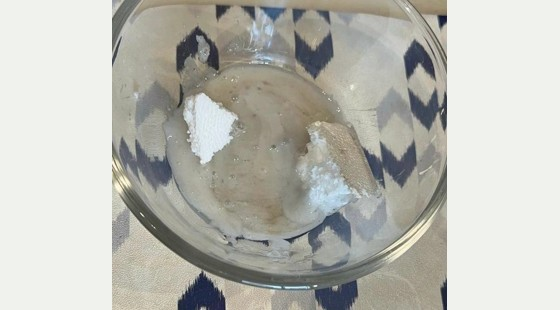
\includegraphics[width=\linewidth,height=4cm]{dissolving.jpg}\\[2pt]
{\small\bfseries Foam dissolving in the peel-derived solvent}\end{minipage}\hfill
\begin{minipage}[t]{0.48\textwidth}\centering
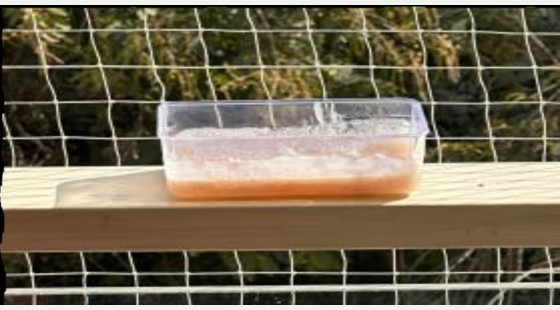
\includegraphics[width=\linewidth,height=4cm]{curing.jpg}\\[2pt]
{\small\bfseries Moulded sample during curing}\end{minipage}

\subsection{Testing the wall design}
For the wall trials, we plan to use a mould that forms air cavities and apply
the white finish to the outward-facing surface. We will weigh each brick
during curing until its mass stabilises and measure how much solvent we
recover for reuse.

\subsection{Experiment: which sample warms up more slowly in sunlight?}
\begin{center}
\begin{tabularx}{\textwidth}{@{}>{\bfseries}p{4.3cm}X@{}}
\toprule
Independent variable & Brick type: CoolBrick or clay brick \\
Dependent variables & Temperature of the back face and the front face \\
Control variables & Thickness and face size, supports, direction, start temperature, probes \\
\bottomrule
\end{tabularx}
\end{center}
We will use one cured CoolBrick sample and one clay-brick sample of the same
thickness and face size. We will tape a contact thermometer probe to the
centre of each back face and a second probe to each front face, and let both
samples reach the same starting temperature in the shade.

We will then stand the samples side by side on identical supports with their
front faces towards the sun and their back probes shaded, and record all four
readings every 10 minutes for \textbf{4 hours}. Heat takes hours to travel
through a brick, so a shorter test would show little change on either back
face. We predict a cooler front face and a smaller temperature rise on the
back of the CoolBrick. We will repeat the test on two more sunny days,
swapping positions between trials.

\subsection{Computer simulation}
We modelled heat moving through each wall minute by minute on a sunny day when
the outdoor air reached 41\,\textdegree C. The simulation held indoor air at 25\,\textdegree C. We
compared peak exterior surface temperature and the heat entering a small model
building over one day.
An animated explanation of the simulation is available at
\url{https://youtu.be/kSh3PBh7VoA}.

% =========================================================================
\section{Results so far achieved and explanation of results}
\subsection{Prototype observations}
\noindent\pic{water.jpg}{Water test}\hfill
\pic{heat.jpg}{Heat test}\hfill
\pic{load.jpg}{Load test}

The cured sample floated during the water check, kept its shape during the
heat check and supported the applied load. These observations show that the
waste-derived gel can form a solid piece that can be handled and tested.
Water uptake, exposure temperature and breaking load still need to be measured.

\subsection{Simulation results}
\begin{center}
\begin{tabularx}{\textwidth}{@{}X>{\centering\arraybackslash}p{3cm}>{\centering\arraybackslash}p{3.8cm}@{}}
\toprule
\bfseries Modelled outcome & \bfseries Clay brick & \bfseries Poly Citra CoolBrick \\
\midrule
Peak outside wall temperature & 52\,\textdegree C & \textbf{39\,\textdegree C} \\
Heat entering the model building over one day, relative to clay & 100\% & \textbf{17\%} \\
\bottomrule
\end{tabularx}
\end{center}

\begin{figure}[H]
\centering
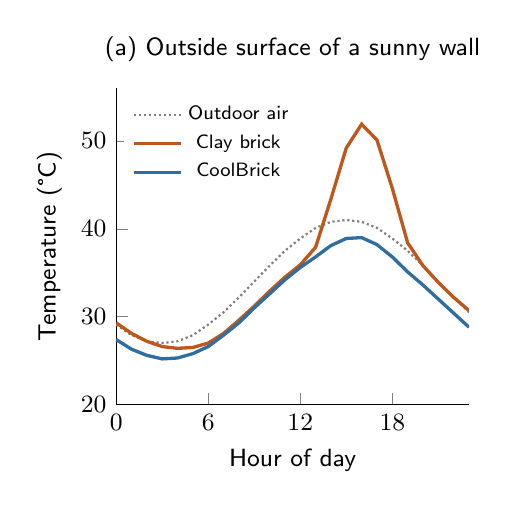
\begin{tikzpicture}
\begin{axis}[width=0.5\textwidth,height=5.6cm,xmin=0,xmax=23,ymin=20,ymax=56,xtick={0,6,12,18},
  xlabel={Hour of day},ylabel={Temperature (\textdegree C)},label style={font=\small},tick label style={font=\small},
  title={\small (a) Outside surface of a sunny wall},
  legend style={font=\scriptsize,at={(0.02,0.98)},anchor=north west,draw=none},axis lines*=left]
\addplot[gray,densely dotted,thick] coordinates {(0,29.1)(1,27.9)(2,27.2)(3,27)(4,27.2)(5,27.9)(6,29.1)(7,30.5)(8,32.2)(9,34)(10,35.8)(11,37.5)(12,38.9)(13,40.1)(14,40.8)(15,41)(16,40.8)(17,40.1)(18,38.9)(19,37.5)(20,35.8)(21,34)(22,32.2)(23,30.5)};\addlegendentry{Outdoor air}
\addplot[accent,very thick] coordinates {(0,29.3)(1,28.1)(2,27.2)(3,26.6)(4,26.4)(5,26.5)(6,27)(7,28.1)(8,29.6)(9,31.2)(10,32.9)(11,34.5)(12,35.9)(13,37.9)(14,43.4)(15,49.2)(16,51.9)(17,50.1)(18,44.6)(19,38.4)(20,35.8)(21,33.9)(22,32.2)(23,30.7)};\addlegendentry{Clay brick}
\addplot[blue,very thick] coordinates {(0,27.4)(1,26.3)(2,25.6)(3,25.2)(4,25.3)(5,25.8)(6,26.6)(7,27.9)(8,29.3)(9,31)(10,32.6)(11,34.2)(12,35.6)(13,36.8)(14,38.1)(15,38.9)(16,39)(17,38.2)(18,36.8)(19,35.1)(20,33.6)(21,32)(22,30.4)(23,28.8)};\addlegendentry{CoolBrick}
\end{axis}
\end{tikzpicture}\hfill
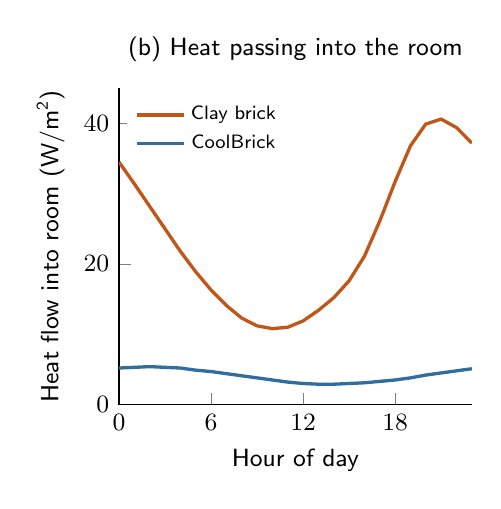
\begin{tikzpicture}
\begin{axis}[width=0.5\textwidth,height=5.6cm,xmin=0,xmax=23,ymin=0,ymax=45,xtick={0,6,12,18},
  xlabel={Hour of day},ylabel={Heat flow into room (W/m\textsuperscript{2})},label style={font=\small},tick label style={font=\small},
  title={\small (b) Heat passing into the room},
  legend style={font=\scriptsize,at={(0.02,0.98)},anchor=north west,draw=none},axis lines*=left]
\addplot[accent,very thick] coordinates {(0,34.5)(1,31.4)(2,28.2)(3,25)(4,21.8)(5,18.9)(6,16.3)(7,14.1)(8,12.3)(9,11.2)(10,10.8)(11,11)(12,11.9)(13,13.4)(14,15.2)(15,17.6)(16,21.1)(17,26.1)(18,31.7)(19,36.8)(20,39.9)(21,40.6)(22,39.4)(23,37.2)};\addlegendentry{Clay brick}
\addplot[blue,very thick] coordinates {(0,5.2)(1,5.3)(2,5.4)(3,5.3)(4,5.2)(5,4.9)(6,4.7)(7,4.4)(8,4.1)(9,3.8)(10,3.5)(11,3.2)(12,3)(13,2.9)(14,2.9)(15,3)(16,3.1)(17,3.3)(18,3.5)(19,3.8)(20,4.2)(21,4.5)(22,4.8)(23,5.1)};\addlegendentry{CoolBrick}
\end{axis}
\end{tikzpicture}
\caption{Computer simulation of a sun-facing (west) wall on a 41\,\textdegree C day, with indoor air held at 25\,\textdegree C. In (b), the heat through the clay wall peaks at night, hours after the sun has hit it, because heat travels slowly through a brick.}
\end{figure}

\subsection{What the results mean}
At its hottest, the modelled CoolBrick surface was 13\,\textdegree C cooler than the clay
surface. For every 100 units of heat entering the clay-brick building over the
day, 17 entered the CoolBrick building. The reflective face reduces solar
heating, while the air pockets slow heat transfer through the wall.

The simulation held indoor air at a fixed temperature. Our sunlight test will
show how much the back of each sample warms during exposure. Estimating the
effect on classroom air temperature would require a separate building-scale test.

\subsection{Will the brick be strong enough?}
Air pockets leave less solid material to carry a load. A laboratory will
measure the force each specimen withstands before failure. Dividing that force
by the loaded face area gives compressive strength in N/mm\textsuperscript{2}.
The lowest class of clay brick in the Indian standard must reach 3.5\,N/mm\textsuperscript{2}
[6]. Published studies of sand bound with dissolved Styrofoam report about
4--12\,N/mm\textsuperscript{2} [5], so a waste-plastic brick can reach this level.
We will also measure water uptake after 24 hours (the standard allows at most
20\%) and arrange fire-performance testing.

% =========================================================================
\section{Conclusion (Details of the outcome of the project)}
\begin{itemize}[leftmargin=*,itemsep=3pt]
  \item \textbf{Outcome 1:} D-limonene from orange peel turns bulky Styrofoam
        into a gel that cures into a solid brick sample, with no kiln.
  \item \textbf{Outcome 2:} the sample floats, keeps its shape when heated and
        supports a load.
  \item \textbf{Outcome 3:} in our computer model, a CoolBrick wall with a white
        face and air pockets stayed 13\,\textdegree C cooler on the outside and let in
        about 80\% less heat than a clay brick wall.
\end{itemize}
These results support the idea that two wastes can make a brick that slows
heat entering a building. They are early results: the sunlight test, water
uptake and strength measurements will show whether real bricks match the model.

% =========================================================================
\section{Future Potential of the Project}
\begin{itemize}[leftmargin=*,itemsep=3pt]
  \item \textbf{Where it could be used:} sun-facing walls in government
        schools, anganwadis and low-cost homes in hot cities such as Delhi.
  \item \textbf{Cost:} our estimate is about \textbf{₹24 per brick}, assuming
        batch production and 90\% solvent recovery; both assumptions need
        checking in production trials. Because this is more than a clay brick
        (₹5--12), it makes most sense on the sunniest walls, funded through
        school grants (Samagra Shiksha) or company CSR funds.
  \item \textbf{Next steps:} run the sunlight test; measure strength, water
        uptake and fire performance; then build a sun-facing test wall at a
        Delhi school to see how it withstands summer heat in use.
\end{itemize}

% =========================================================================
\section{Bibliography, References and Acknowledgements}
\subsection{References}
\small
\begin{enumerate}[label={[\arabic*]},leftmargin=*,itemsep=1pt]
\item Park, R.\,J., Goodman, J., Hurwitz, M.\ \& Smith, J.\ (2020). Heat and Learning. \emph{American Economic Journal: Economic Policy}, 12(2), 306--339.
\item Ministry of Education (2024). \emph{UDISE+ 2023--24}. Government of India.
\item Li, X.\ et al.\ (2020). Full daytime sub-ambient radiative cooling in commercial-like paints. \emph{Cell Reports Physical Science}, 1(10).
\item Florida Chemical Company. D-limonene as a solvent for expanded polystyrene; Sony Corporation, limonene-based polystyrene recycling.
\item Assessing the feasibility of using EPS mortar as a construction material for mitigating foam waste. \emph{TNI Journal of Engineering and Technology}.
\item Bureau of Indian Standards. IS 1077 (common burnt clay building bricks) and IS 3495 (methods of tests of burnt clay bricks).
\end{enumerate}
\normalsize

\subsection{Acknowledgements}
\textbf{Original project credit.} Daiwik Abrol and his sister, Prisha Abrol,
developed the original brick prototype using discarded Styrofoam and orange
peels. Daiwik and Rian Sikka built on that work by developing the CoolBrick
wall design and planning a sunlight test to compare it with a clay brick.

We thank Scottish High International School and our teachers for laboratory
access and guidance, and our families for their support.

\end{document}
